\chapter*{Úvod}
\addcontentsline{toc}{chapter}{Úvod}

Slávna Eulerova úloha siedmych mostov v Kaliningrade \cite{euler41} sa považuje za prvú prácu, 
ktorá zaviedla teóriu grafov.
Úlohou je prejsť po týchto siedmych mostoch tak, aby sme po každom šli práve raz.


\begin{figure}[h]
\centering
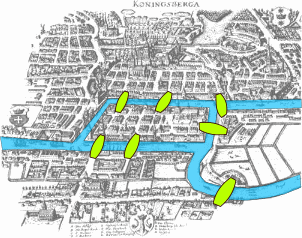
\includegraphics[height=7.5cm]{./img/Konigsberg_bridges.png}
\caption{Sedem mostov v Kaliningrade}
\label{fig:konigsberg_bridges}
\end{figure}


 
Od tej doby sa využitie teórie grafov značne
rozšírilo a v dnešnej dobe patrí medzi významné
a rozpracované teórie. V modernej dobe je jedným z jej 
najdôležitejších problémov hľadanie najkratšej cesty. Najčastejšie sa s nimi stretávame pri plánovaní trasy v
GPS navigácii.
Medzi najvýznamnešie práce považujeme práce od Dijkstru \cite{dijkstra59} a Floyd-Warshalla.

S narastajúcim fenoménom počítačových hier 
a umelej inteligencie sa do povedomia dostal špeciálny typ grafu --
mriežkový graf, využívaný ako herná mapa.
V hrách často trebalo nájsť cestu pre počítačom
ovládanú postavičku z miesta A do miesta B.
Nakoľko je väčšina hier komerčná, algoritmy
využívané v hrách boli a sú taktiež komerčné.
Dôsledkom toho nie sú verejne publikované a porovnané rôzne prístupy a algoritmy
na vyhľadávanie najkratších ciest v mriežkových mapách. A keď už aj sú, tak práce používajú rôzne mapy
na bechmarking a teda neexistuje žiadna globálna porovnávacia štúdia týchto prístupov.

Súťaž {\sl Grid-Based Path Planning Competition}
 \cite{sturtevantgppc} sa snaží tento problém vyriešiť tým, že porovnáva rôzne algoritmy na veľkej množine máp
použitých v známych počítačových hrách a vyhodnocuje ich úspešnosť v rámci viacerých kategórií.

Cieľom tejto práce je spraviť prehľad doterajších prístupov k tomuto problému a prispieť vlastným algoritmom do sútaže a niekoľkými vylepšeniami k doterajším prístupom hľadania najkratšej cesty na mriežkových grafoch.

V prvej kapitole si zavedieme kľúčové termíny a popíšeme problém formálne. Na konci kapitoly spomenieme súťaž, ktorej sa daný algoritmus zúčastnil.

Druhá kapitola je zameraná na vytvorenie prehľadu kľúčových algoritmov použivaných na riešenie problému.

V tretej kapitole navrhneme vlastné riešenie založené na poznatkoch popísaných v druhej kapitole s pridaním vlastných vylepšení.

Vo štvrtej kapitole toto riešenie porovnáme s dosavadnými.


